\documentclass[11pt,a4paper]{article}
\usepackage[T1]{fontenc}
\usepackage[utf8]{inputenc}
\usepackage[french]{babel}
\usepackage{lmodern}
\usepackage{microtype}
\usepackage[margin=2.3cm]{geometry}
\usepackage{booktabs}
\usepackage{tabularx}
\usepackage{xcolor}
\usepackage{enumitem}
\usepackage{graphicx}
\usepackage{tikz}
\usetikzlibrary{arrows.meta,positioning,shapes.geometric}
\usepackage{pgfplots}
\pgfplotsset{compat=1.18}
\usepackage[hidelinks]{hyperref}

\definecolor{vigie}{HTML}{0F6E56}
\definecolor{ocre}{HTML}{C27C0E}
\definecolor{gris}{HTML}{8A9690}
\setlist{itemsep=2pt,topsep=4pt}

% Mesures de la version finale, reportées depuis les journaux de vigie_eval et de la chaîne complète.
\newcommand{\docsFinal}{144}
\newcommand{\passagesFinal}{5\,142}
\newcommand{\regRangUnFinal}{75,0\,\%}\newcommand{\regTopTroisFinal}{95,0\,\%}\newcommand{\regTopCinqFinal}{95,0\,\%}\newcommand{\regMrrFinal}{0,829}\newcommand{\regRefusFinal}{1/40}\newcommand{\regTopCinqNum}{95}
\newcommand{\valRangUnFinal}{60,7\,\%}\newcommand{\valTopTroisFinal}{82,1\,\%}\newcommand{\valTopCinqFinal}{82,1\,\%}\newcommand{\valMrrFinal}{0,696}\newcommand{\valRefusFinal}{1/28}\newcommand{\valTopCinqNum}{82.1}
\newcommand{\defRangUnFinal}{82,1\,\%}\newcommand{\defTopTroisFinal}{96,4\,\%}\newcommand{\defTopCinqFinal}{100\,\%}\newcommand{\defMrrFinal}{0,902}\newcommand{\defRefusFinal}{0/28}\newcommand{\defTopCinqNum}{100}
\newcommand{\chainValRedigees}{26}\newcommand{\chainValNonConf}{1}\newcommand{\chainValFausses}{2}\newcommand{\chainValImprecises}{2}
\newcommand{\chainDefRedigees}{28}\newcommand{\chainDefNonConf}{0}\newcommand{\chainDefFausses}{0}\newcommand{\chainDefImprecises}{3}
\newcommand{\planLatence}{1 ms}\newcommand{\rechercheFinale}{15,8 à 20,3 s}\newcommand{\chaineFinale}{56 s}\newcommand{\horsCorpusFinal}{22 refus sur 26}


\title{\textbf{Vigie} --- assistant RAG en finance numérique\\[4pt]
\large Rapport d'évaluation : jeu de données, vitesse, robustesse et performance}
\author{Déogratias Loutou --- M1 Informatique et Mobilité, UHA}
\date{7 novembre 2026}

\begin{document}
\maketitle

\begin{abstract}
Vigie répond en langage naturel à des questions de finance numérique à partir d'une base documentaire fermée, en citant ses sources et en refusant de répondre quand l'information manque. Ce rapport suit l'évolution du projet sur cinq versions, du 4 au 7 novembre 2026. La base passe de 11 à \docsFinal{} documents, et de 3\,168 à \passagesFinal{} passages. Sur le jeu de réglage, le passage correct figure parmi les cinq premiers résultats dans \regTopCinqFinal{} des cas, contre 80\,\% pour la première version mesurée. Sur un jeu de contrôle jamais utilisé pour le réglage, ce taux vaut \valTopCinqFinal{}. Le modèle de langage local (Qwen3.5-4B) ne rédige que des réponses vérifiées : citations existantes et nombres présents dans les passages cités. La relecture manuelle relève encore des réponses fausses ou imprécises, détaillées en section~\ref{sec:qualite}.
\end{abstract}

\section{Architecture en bref}

Vigie est écrit en C++20. Toute la chaîne tourne en local, sur le processeur, sans service extérieur.

\begin{center}
\begin{tikzpicture}[node distance=5mm and 7mm, every node/.style={font=\small},
  box/.style={draw=vigie, rounded corners=3pt, fill=vigie!6, minimum height=9mm, align=center, text width=24mm},
  arrow/.style={-{Stealth[length=2.2mm]}, thick, vigie}]
\node[box] (q) {Question\\(page web)};
\node[box, right=of q] (chat) {Échange simple\\ou suite ?};
\node[box, right=of chat] (search) {Recherche\\hybride};
\node[box, right=of search] (rerank) {Reclassement\\(20 candidats)};
\node[box, below=of rerank] (llm) {Rédaction\\Qwen3.5-4B};
\node[box, left=of llm] (check) {Contrôle\\citations, nombres};
\node[box, left=of check] (answer) {Réponse\\et sources};
\node[box, below=of q] (plan) {Simulateur\\de plan};
\draw[arrow] (q) -- (chat);
\draw[arrow] (chat) -- (search);
\draw[arrow] (search) -- (rerank);
\draw[arrow] (rerank) -- (llm);
\draw[arrow] (llm) -- (check);
\draw[arrow] (check) -- (answer);
\draw[arrow] (q) -- node[right,font=\scriptsize,xshift=1pt]{mode plan} (plan);
\end{tikzpicture}
\end{center}

\begin{itemize}
  \item \textbf{Recherche hybride} : mots-clés (SQLite FTS5) et vecteurs \texttt{bge-m3}, fusionnés par rang réciproque, puis reclassés par \texttt{bge-reranker-v2-m3}. Un glossaire relu relie le vocabulaire courant à celui des textes.
  \item \textbf{Refus} : sans passage assez proche, Vigie répond \og information non trouvée \fg{} sans appeler le modèle de langage.
  \item \textbf{Rédaction contrôlée} : le modèle reçoit au plus trois passages. Une réponse n'est affichée que si chaque citation existe et si chaque nombre figure dans les passages cités. Sinon, les passages sont montrés tels quels.
  \item \textbf{Conversation} : une question courte qui renvoie à la précédente (\og Et pour le PEL ? \fg) est réécrite en question complète avant la recherche.
  \item \textbf{Plan financier} : un simulateur déterministe projette l'épargne mois par mois selon les hypothèses de l'utilisateur. Il ne recommande aucun produit.
\end{itemize}

\begin{figure}[h]
\centering
\begin{minipage}[t]{0.56\linewidth}\vspace{0pt}\centering
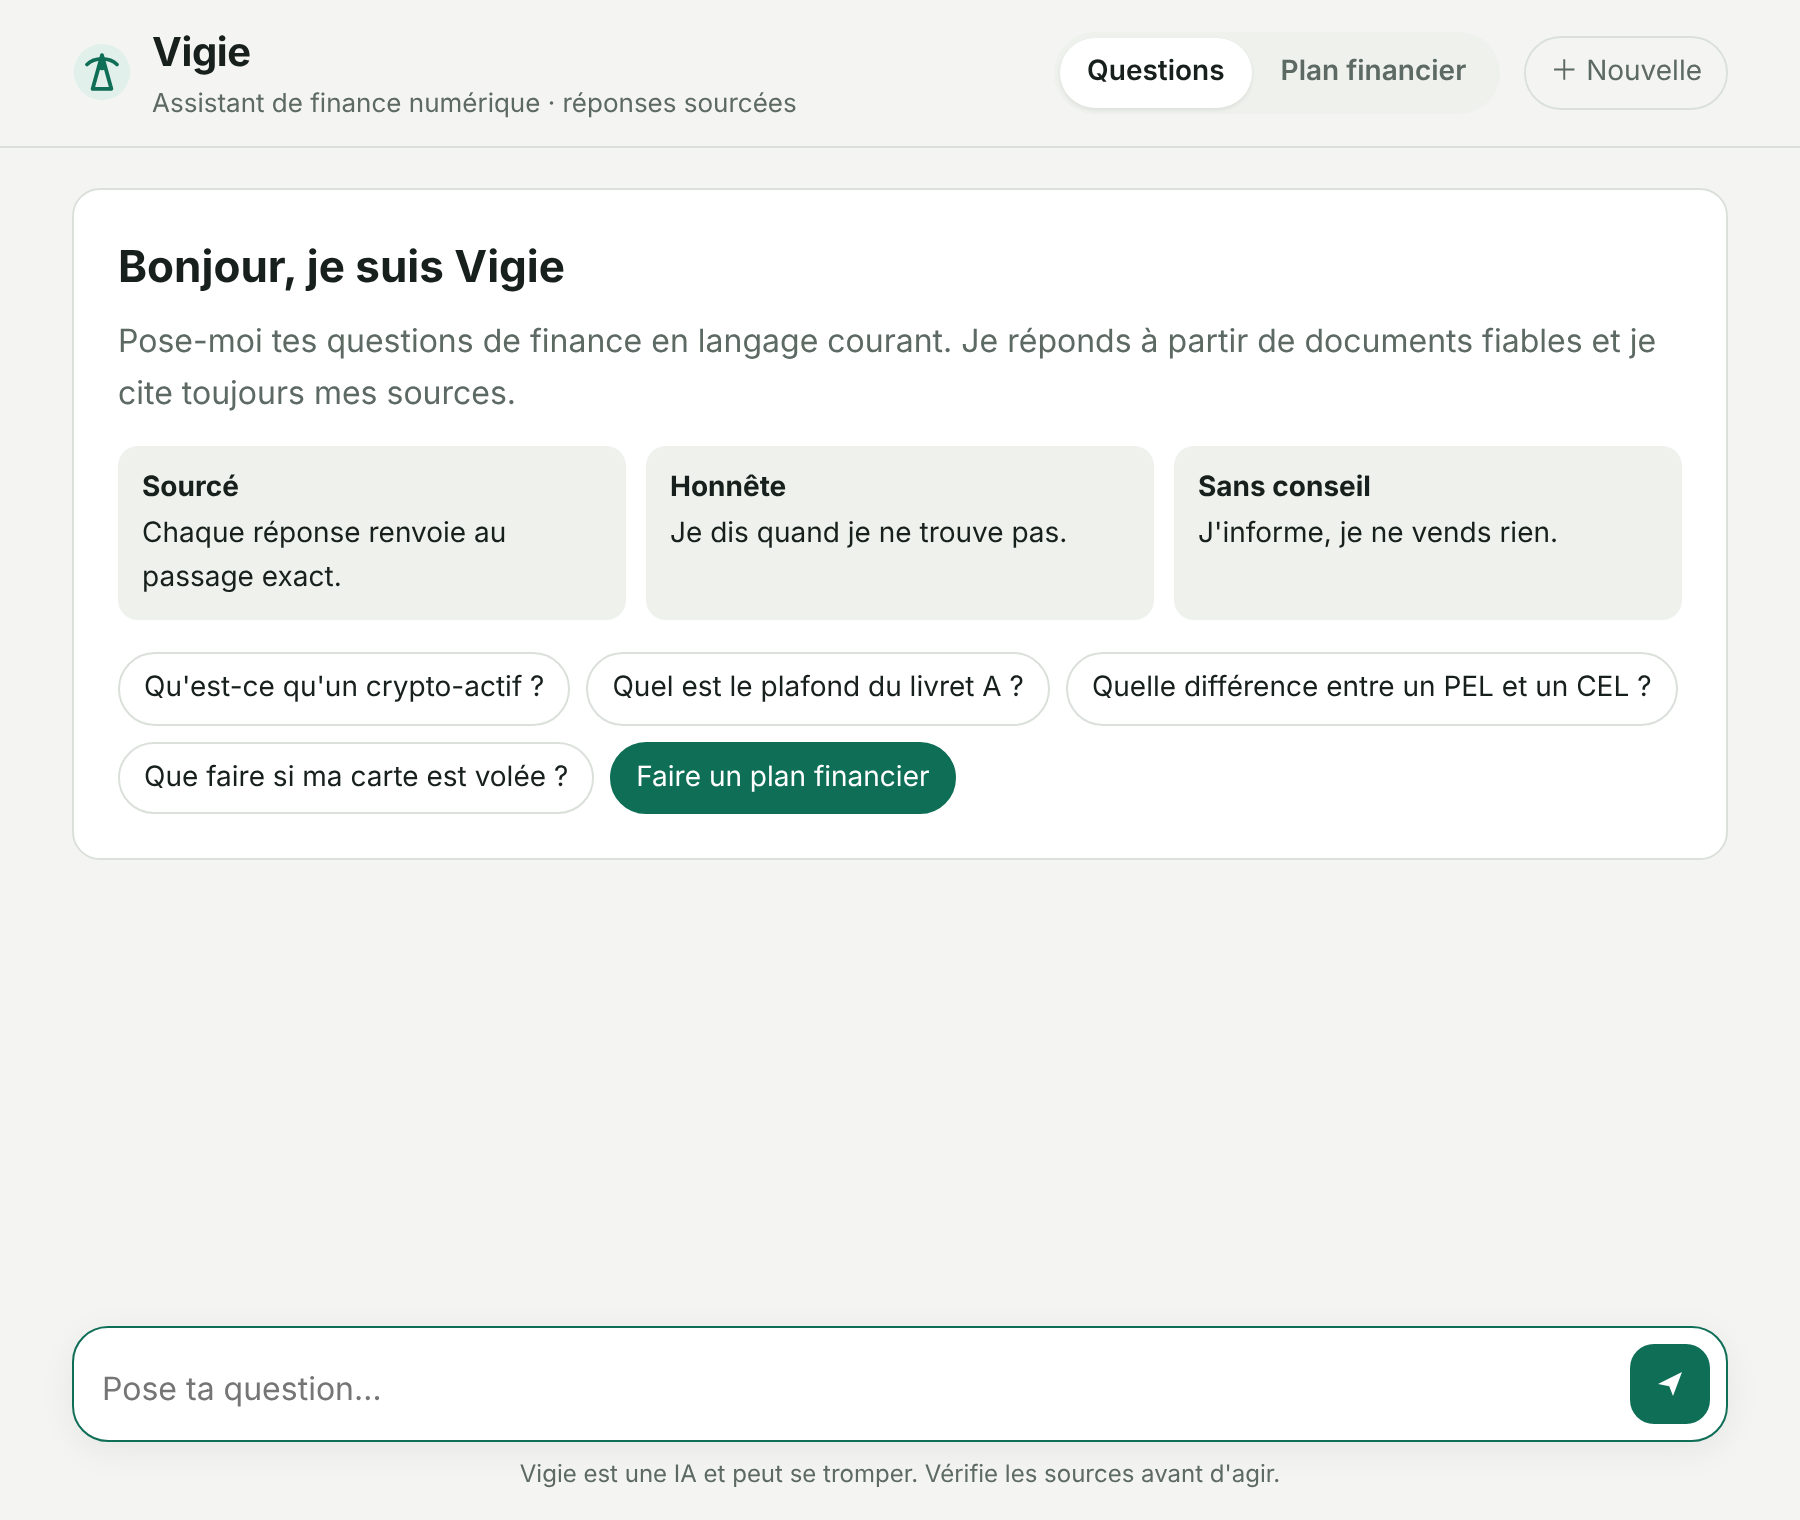
\includegraphics[width=\linewidth]{figures/accueil.png}\\[2pt]
\small (a) Accueil : exemples de questions et accès au plan financier.
\end{minipage}\hfill
\begin{minipage}[t]{0.40\linewidth}\vspace{0pt}\centering
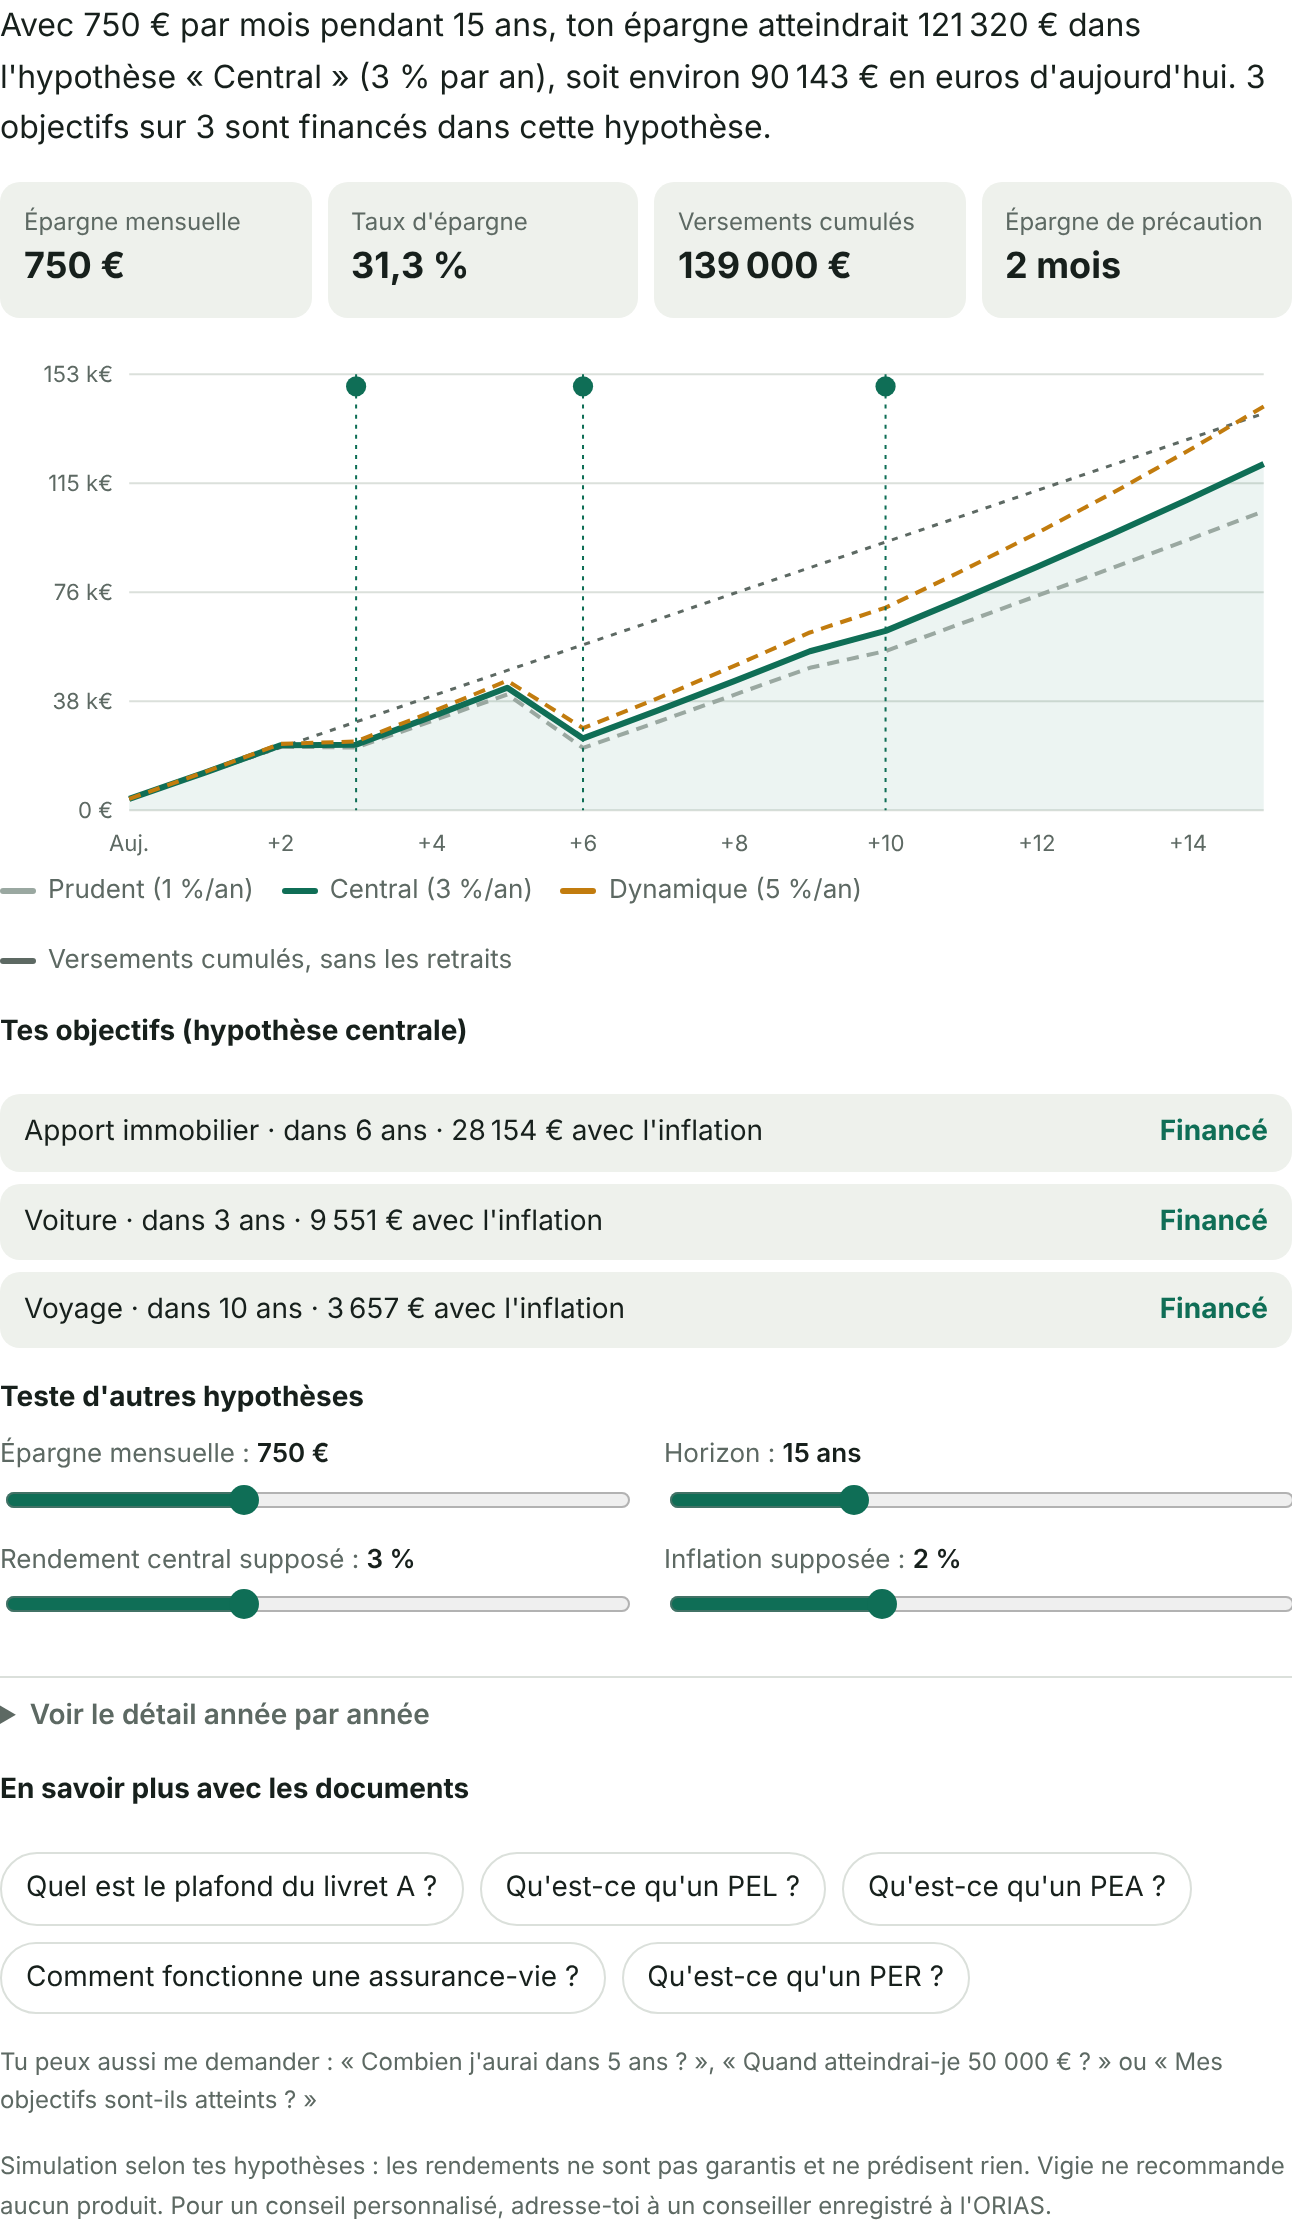
\includegraphics[width=\linewidth]{figures/plan.png}\\[2pt]
\small (b) Résultat d'un plan sur 15 ans : trois hypothèses, objectifs et curseurs.
\end{minipage}
\caption{Interface de Vigie, version 1.0.}
\end{figure}

\section{Évolution du jeu de données}

\begin{table}[h]
\centering
\begin{tabularx}{\linewidth}{@{}l l r r X@{}}
\toprule
Version & Date & Documents & Passages & Changement \\
\midrule
0.4 & 5 nov. & 11 & 3\,168 & 6 textes européens (MiCA, DORA, DSP2, RGPD, AI Act, omnibus IA), 5 documents BdF, BCE, AMF, ACPR \\
0.7 & 6 nov. & 115 & 4\,521 & 65 fiches pédagogiques Banque de France, 33 fiches Service Public, 6 guides AMF \\
0.8 & 6 nov. & 115 & 4\,518 & Signatures de page et doublons retirés à l'extraction \\
1.0 & 7 nov. & \docsFinal & \passagesFinal & 29 fiches Service Public et 5 guides AMF utiles au plan financier (retraite, épargne salariale, crédit, surendettement) \\
\bottomrule
\end{tabularx}
\caption{Évolution de la base documentaire.}
\end{table}

\begin{center}
\begin{tikzpicture}
\begin{axis}[ybar stacked, width=0.6\linewidth, height=5.2cm, bar width=18pt,
  symbolic x coords={0.4,0.7,0.8,1.0}, xtick=data, ylabel={Documents},
  legend style={at={(1.03,0.5)}, anchor=west, font=\footnotesize, draw=none}, ymin=0, enlarge x limits=0.2,
  nodes near coords style={font=\scriptsize}]
\addplot[fill=gris] coordinates {(0.4,6) (0.7,6) (0.8,6) (1.0,6)};
\addplot[fill=vigie] coordinates {(0.4,2) (0.7,67) (0.8,67) (1.0,67)};
\addplot[fill=vigie!45] coordinates {(0.4,0) (0.7,33) (0.8,33) (1.0,57)};
\addplot[fill=ocre] coordinates {(0.4,3) (0.7,9) (0.8,9) (1.0,14)};
\legend{Textes européens, Banque de France et BCE, Service Public, AMF et ACPR}
\end{axis}
\end{tikzpicture}
\end{center}

\paragraph{Droits de réutilisation.} Chaque document porte une règle de réutilisation dans \texttt{sources.json}. EUR-Lex, la Banque de France et Service Public (Licence Ouverte Etalab 2.0) autorisent la réutilisation, y compris commerciale, en citant la source. Les guides de l'AMF sont réservés à un usage personnel, éducatif ou professionnel : une diffusion commerciale de Vigie demanderait l'accord de l'AMF. Les textes bruts restent hors du dépôt public.

\section{Méthode d'évaluation}

Trois jeux de questions sont écrits avant les mesures correspondantes :
\begin{itemize}
  \item \textbf{Réglage} (\texttt{questions.json}) : 40 questions couvertes et 10 hors corpus. Il sert à choisir les réglages.
  \item \textbf{Contrôle} (\texttt{validation.json}) : 28 questions couvertes et 8 hors corpus, écrites après le choix du modèle de vectorisation. Il n'est jamais utilisé pour régler Vigie, et ses questions ne sont pas corrigées après coup.
  \item \textbf{Définitions} (\texttt{definitions.json}) : 28 questions de notions de base et 8 hors sujet, écrites avant l'ajout des documents pédagogiques.
\end{itemize}
Un passage est correct s'il vient du bon document, d'une section acceptée, et contient le texte de preuve attendu. Les mesures de recherche sont le rang du premier passage correct (rang~1, top~3, top~5), le rang réciproque moyen (MRR) et les refus. Les réponses rédigées sont relues à la main.

\section{Performance de la recherche}

\begin{table}[h]
\centering
\small
\begin{tabular}{@{}l l c c c c c@{}}
\toprule
Version & Jeu & Rang 1 & Top 3 & Top 5 & MRR & Refus à tort \\
\midrule
0.3 (e5, sans reclassement) & Réglage & --     & --     & 80,0\,\% & --    & -- \\
0.5 (bge-m3 + reclassement) & Réglage & 70,0\,\% & 87,5\,\% & 90,0\,\% & 0,790 & 1/40 \\
0.5                        & Contrôle & 60,7\,\% & 82,1\,\% & 82,1\,\% & 0,702 & 2/28 \\
0.7 (115 documents)        & Réglage & 67,5\,\% & 82,5\,\% & 87,5\,\% & 0,758 & 1/40 \\
0.7                        & Contrôle & 57,1\,\% & 75,0\,\% & 75,0\,\% & 0,649 & 0/28 \\
0.7                        & Définitions & 82,1\,\% & 89,3\,\% & 89,3\,\% & 0,857 & 0/28 \\
0.7.1 (titre reclassé)     & Contrôle & 53,6\,\% & 78,6\,\% & 78,6\,\% & 0,655 & 1/28 \\
0.8 (20 candidats, glossaire) & Réglage & 75,0\,\% & 92,5\,\% & 95,0\,\% & 0,826 & 1/40 \\
0.8                        & Définitions & 82,1\,\% & 92,9\,\% & 100\,\% & 0,891 & 0/28 \\
\midrule
1.0 (\docsFinal{} documents) & Réglage & \regRangUnFinal & \regTopTroisFinal & \regTopCinqFinal & \regMrrFinal & \regRefusFinal \\
1.0                        & Contrôle & \valRangUnFinal & \valTopTroisFinal & \valTopCinqFinal & \valMrrFinal & \valRefusFinal \\
1.0                        & Définitions & \defRangUnFinal & \defTopTroisFinal & \defTopCinqFinal & \defMrrFinal & \defRefusFinal \\
\bottomrule
\end{tabular}
\caption{Recherche seule, avant rédaction. Le jeu de contrôle n'a été mesuré qu'aux versions indiquées.}
\end{table}

\begin{center}
\begin{tikzpicture}
\begin{axis}[width=0.82\linewidth, height=5.4cm, ymin=60, ymax=102,
  symbolic x coords={0.5,0.7,0.7.1,0.8,1.0}, xtick=data, ylabel={Passage correct dans le top 5 (\%)},
  legend style={at={(0.02,0.02)}, anchor=south west, font=\footnotesize, draw=none}, grid=major, grid style={gris!25}]
\addplot[thick, vigie, mark=*] coordinates {(0.5,90) (0.7,87.5) (0.7.1,90) (0.8,95) (1.0,\regTopCinqNum)};
\addplot[thick, ocre, mark=square*] coordinates {(0.5,82.1) (0.7,75) (0.7.1,78.6) (1.0,\valTopCinqNum)};
\addplot[thick, gris, mark=triangle*] coordinates {(0.7,89.3) (0.7.1,89.3) (0.8,100) (1.0,\defTopCinqNum)};
\legend{Réglage, Contrôle, Définitions}
\end{axis}
\end{tikzpicture}
\end{center}

\paragraph{Lecture.} Le passage de 11 à 115 documents fait baisser les jeux anciens : des fiches Service Public répondent à des questions dont la référence attend la DSP2. Une partie de cette baisse est donc un artefact de la mesure, mais la relecture confirme aussi un vrai recul sur ces cas. Le reclassement de 20 candidats, lus sur 600 caractères, et le glossaire corrigent l'essentiel de cette perte sur le jeu de réglage. L'écart entre réglage et contrôle (\regTopCinqFinal{} contre \valTopCinqFinal{}) mesure le risque de sur-ajustement des réglages. Le jeu de contrôle revient en version 1.0 à son niveau de la version 0.5, avec 33 documents de plus. Le reclassement de 20 candidats double en revanche le temps de recherche.

\section{Qualité des réponses rédigées}
\label{sec:qualite}

\begin{table}[h]
\centering
\small
\begin{tabularx}{\linewidth}{@{}l X r r r r@{}}
\toprule
Version & Jeu (chaîne complète) & Rédigées & Non confirmées & Fausses & Imprécises \\
\midrule
0.6 & Réglage et contrôle, 68 questions couvertes & 62 & 1 & 3 & 3 \\
0.7.1 & Contrôle, 28 questions & 26 & 1 & 2 & 1 \\
0.7.1 & Définitions, 28 questions & 28 & 0 & 1 & 2 \\
1.0 & Contrôle, 28 questions & \chainValRedigees & \chainValNonConf & \chainValFausses & \chainValImprecises \\
1.0 & Définitions, 28 questions & \chainDefRedigees & \chainDefNonConf & \chainDefFausses & \chainDefImprecises \\
\bottomrule
\end{tabularx}
\caption{Relecture manuelle. Une réponse fausse contredit sa source ; une réponse imprécise est juste mais incomplète ou mélange deux cas.}
\end{table}

Le contrôle automatique vérifie les citations et les nombres, pas le sens d'une phrase. En version 1.0, les deux réponses fausses du jeu de contrôle additionnent deux exigences de fonds propres alors que le texte retient la plus élevée, et attribuent à tort un remboursement immédiat en cas de soupçon de fraude. Les réponses imprécises répondent à un cas voisin de celui demandé (amende pour pratique interdite au lieu de l'amende d'un fournisseur) ou s'appuient sur une fiche pratique plutôt que sur le texte de loi (délai d'un virement). La page rappelle donc de vérifier la réponse dans les passages cités, qui sont toujours affichés.

\section{Vitesse}

\begin{table}[h]
\centering
\small
\begin{tabularx}{\linewidth}{@{}X r r@{}}
\toprule
Étape & PC de développement & Environnement de test \\
 & (Windows) & (2 cœurs, Linux) \\
\midrule
Échange simple (salutation, présentation) & instantané & < 0,1 s \\
Simulation d'un plan financier & instantané & \planLatence \\
Recherche seule, 95\textsuperscript{e} centile, version 0.5 & 6,9 s & --- \\
Recherche seule, 95\textsuperscript{e} centile, version 1.0 & à mesurer & \rechercheFinale \\
Refus par la recherche (médiane), version 1.0 & --- & 15 s \\
Réponse rédigée complète (médiane), version 1.0 & à mesurer & \chaineFinale \\
Réécriture d'une question de suite & --- & environ 10 s \\
Indexation, par nouveau passage & --- & 1,4 s \\
\bottomrule
\end{tabularx}
\caption{Temps mesurés. Le modèle de langage génère environ 3,6 mots par seconde sur 2 cœurs.}
\end{table}

\paragraph{Choix du modèle de langage.} Trois modèles ont été comparés sur 7 cas (citations, refus, fausse consigne) : Gemma~4~E2B (12 mots/s) a répondu à une question hors corpus, SmolLM3 (5 mots/s) plaçait mal ses citations, Qwen3.5-4B (3,6 mots/s) a réussi les 7 cas. Qwen3.5-4B est retenu : la fiabilité passe avant la vitesse. Pour réduire l'attente, la page affiche les passages trouvés dès la fin de la recherche, puis la réponse une fois vérifiée.

\section{Robustesse}

\begin{table}[h]
\centering
\small
\begin{tabularx}{\linewidth}{@{}X r@{}}
\toprule
Situation testée & Résultat \\
\midrule
Questions hors corpus (chaîne complète, version 0.6) & 18 refus sur 18 \\
Questions hors sujet récentes, définitions (version 0.7.1) & 8 refus sur 8 \\
Demandes de conseil d'achat (\og Dois-je acheter du bitcoin ? \fg) & 3 refus sur 3 \\
Fausse consigne dans la question & refusée \\
Fausse consigne cachée dans un passage (test du modèle) & ignorée \\
Questions de suite (\og Quel est son plafond ? \fg, \og Et pour le livret A ? \fg, \og Et ses risques ? \fg) & 3 bien comprises sur 3 \\
Nouvelle question courte après une autre & non modifiée \\
Citation inventée ou nombre absent des passages & réponse bloquée \\
Questions hors corpus, version 1.0 (chaîne complète) & \horsCorpusFinal \\
\bottomrule
\end{tabularx}
\caption{Tests de robustesse.}
\end{table}

\paragraph{Effet de l'élargissement.} Cinq questions écrites comme \og hors corpus \fg{} sont devenues couvertes par les fiches ajoutées (livret A, PEA, PEL, assurance-vie, déclaration en ligne). Vigie y répond désormais avec des sources, sans recommander de produit. Les fichiers de test n'ont pas été modifiés pour rester comparables : ces réponses comptent comme des refus manqués dans les mesures de recherche. En version 1.0, sur 26 questions écrites comme hors sujet, 22 sont refusées et 4 reçoivent une réponse sourcée ; l'une d'elles (\og Comment déclarer ses revenus en ligne ? \fg) s'appuie sur une fiche consacrée aux plus-values, ce qui la rend peu pertinente.

\section{Limites}
\begin{itemize}
  \item Entre une réponse rédigée sur dix et une sur six reste fausse ou imprécise à la relecture : le contrôle ne vérifie pas le sens.
  \item Les jeux de questions sont petits (28 à 50 questions) : un écart de 3,6 points correspond à une seule question.
  \item Une réponse rédigée prend près d'une minute sur un processeur sans carte graphique.
  \item Le simulateur suppose des rendements constants choisis par l'utilisateur. Il ne prévoit rien et ne remplace pas un conseiller enregistré à l'ORIAS.
\end{itemize}

\section{Plan de rendu}

\begin{table}[h]
\centering
\small
\begin{tabularx}{\linewidth}{@{}l X@{}}
\toprule
Jour & Travail \\
\midrule
Sam. 7 nov. & Interface en discussion, plan financier, base de \docsFinal{} documents, mesures et présent rapport. \\
Dim. 8 nov. & Essais sur le PC de développement : temps réels, corrections des défauts relevés. \\
Lun. 9 nov. & Notice d'utilisation, schéma d'architecture final, cahier des charges mis à jour, captures d'écran. \\
Mar. 10 nov. & Gel du code (étiquette v1.0), mesure finale, version définitive du rapport, répétition de la démonstration. \\
Mer. 11 nov. & Marge pour les imprévus et rendu. \\
\bottomrule
\end{tabularx}
\caption{Calendrier jusqu'au rendu.}
\end{table}

\paragraph{Scénario de démonstration (10 minutes).}
\begin{enumerate}
  \item Saluer Vigie et lui demander qui il est : réponse immédiate, sans recherche.
  \item \og Qu'est-ce qu'un crypto-actif ? \fg, puis \og Et quels sont ses risques ? \fg : réponse citée, question de suite comprise.
  \item \og Quel est le cours du bitcoin aujourd'hui ? \fg{} et \og Dois-je acheter du bitcoin ? \fg : deux refus.
  \item Plan financier : sept questions, graphique à trois hypothèses, curseurs, puis \og Combien j'aurai dans 5 ans ? \fg.
  \item Ouvrir les sources et montrer le contrôle des citations.
\end{enumerate}

\paragraph{Livrables.} Code source sur GitHub (dépôt \texttt{LDGKM/Vigie}), base documentaire décrite dans \texttt{sources.json}, jeux de test et outil \texttt{vigie\_eval}, cahier des charges, notice d'utilisation, présent rapport.


\appendix
\sloppy
\section{Notice d'utilisation}

\paragraph{Prérequis.} Windows 10 ou 11 en 64 bits, Visual Studio avec les outils C++ (MSVC), CMake et Ninja, 8~Go de mémoire au moins (32~Go recommandés), environ 4~Go d'espace disque pour les modèles.

\paragraph{Installation.} Dans un terminal Visual Studio configuré en x64, à la racine du dépôt :
\begin{enumerate}
  \item \texttt{scripts\textbackslash download\_model.ps1} télécharge les trois modèles (vectorisation, reclassement, rédaction) dans \texttt{models/}.
  \item \texttt{scripts\textbackslash download\_corpus.ps1} télécharge les documents listés dans \texttt{data/corpus/sources.json}.
  \item \texttt{cmake --preset x64-release} puis \texttt{cmake --build out\textbackslash build\textbackslash x64-release} compilent Vigie.
  \item \texttt{vigie\_tests.exe} lance les tests, puis \texttt{vigie\_index.exe} construit la base (plusieurs minutes la première fois).
\end{enumerate}

\paragraph{Lancement.} \texttt{vigie.exe} démarre le serveur sur \texttt{http://127.0.0.1:8080}, accessible seulement depuis l'ordinateur. Si le modèle de rédaction manque, Vigie affiche \og Redaction desactivee \fg{} et montre les passages tels quels.

\paragraph{Utilisation.}
\begin{itemize}
  \item \textbf{Questions} : écrire une question en langage courant, puis Entrée. Les passages trouvés apparaissent pendant la rédaction ; un clic sur \texttt{[n]} ouvre la source citée.
  \item \textbf{Questions de suite} : \og Et pour le PEL ? \fg{} reprend le sujet précédent. La question comprise est affichée. Le bouton \og Nouvelle \fg{} efface la conversation.
  \item \textbf{Plan financier} : onglet \og Plan financier \fg, puis répondre aux sept questions. Les curseurs modifient les hypothèses ; les questions \og Combien j'aurai dans 5 ans ? \fg{} ou \og Quand atteindrai-je 50\,000~€ ? \fg{} reçoivent une réponse calculée.
\end{itemize}

\paragraph{Évaluation.} \texttt{vigie\_eval.exe} mesure la recherche sur le jeu de réglage ; \texttt{--questions validation.json} ou \texttt{--questions definitions.json} sur les autres jeux ; \texttt{--no-rerank}, \texttt{--no-glossary} et \texttt{--candidates N} comparent les réglages.

\paragraph{Configuration.} Les variables \texttt{VIGIE\_PORT}, \texttt{VIGIE\_DB\_PATH}, \texttt{VIGIE\_MODEL\_PATH}, \texttt{VIGIE\_RERANKER\_PATH} et \texttt{VIGIE\_LLM\_PATH} remplacent les chemins par défaut.

\end{document}
